\qns{Energy Disaggregation - EXAMPLE}

This is where you write the main question
\begin{enumerate} % This is important to start parts. Thenceforth use \qitem, \ans{} and \sol{}.
\qitem This is where you write part (a) \\ Hello
\ans{
This is where you write student solutions
}

\sol{
This is where you write mentor solutions
}

\qitem This is where you write part (b)
% This is how you insert a figure (image figure!)
\begin{figure}[H]
	\begin{center}
		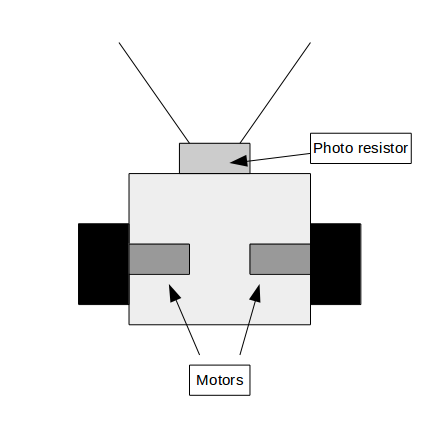
\includegraphics[scale=0.35]{figures/PetBot1.png}
	\end{center}
\end{figure}

\ans{
This is where you write student solution

\begin{align*}
x_{\text{R}} & = T_1 \\
x_{\text{AC}} + x_{\text{TV}} + x_{\text{R}} & = T_2 \\
x_{\text{AC}} + x_{\text{R}} & = T_3
\end{align*}
}

\sol{
This is where you write mentor solutions. 
}

\qitem This is where you write part (c)
% This is how you insert in-line circuitikz
\begin{center}
	\begin{circuitikz}
		% \draw[help lines] (0,0) to (5,5);
		\draw (2, 2)
		node[op amp, yscale=-1] (comp){};
		\draw (comp.out) |- (3, -0.5);
		\draw (comp.out)
		to[short,-o] ++(1,0)
		node[right]{$v_\text{out}$};
		\draw (3, -0.5)
		to[short] ++(-2,0);
		\draw (1,-0.5) -| (comp.-);
		\draw (-1,2)
		to[short] ++(0.5,0);
		\draw (-0.5,2) |- (comp.+);
		\draw (comp.down) % note that down is actually the top rail because we flipped this
		to ++(0,0.5) node [above]{\SI{10}{\volt}};
		\draw (comp.up)
		to ++(0,-0.5) node [ground]{};
		\draw (-1,0)
		to[phR] ++(0,2)
		to[R,l=$R$] ++(0,2)
		to[short] ++(-1.5,0);
		\draw (-1,0)
		node[ground]{};
		\draw (-2.5,0)
		to[V,l=$\SI{10}{\volt}$, invert] ++(0,4);
		\draw (-2.5,0)
		node[ground]{};
		
	\end{circuitikz}
\end{center}

\ans{
	Student solution here \\

	% This is how you define an equation so it automatically gets a number
	\begin{equation} \label{q_lindep:eq:given}
	\alpha_1 \cdot \vec{v}_1 + \alpha_2 \cdot \vec{v}_2 + \dots + \alpha_k \cdot \vec{v}_k = \vec{0}.
	\end{equation}

	% This is how you refer to equations
	Equation \ref{q_lindep:eq:given} is the great equation
}

%NOTE: There is no TA solution.


\end{enumerate}
